\documentclass{article}
\usepackage[utf8]{inputenc}
\usepackage{graphicx}
\usepackage{float}
\graphicspath{{figures/}}

\title{Classification of Tweets into Various Categories using Naive Bayes Classification Algorithm}
\author{Diana-Isabela \textbf{Crainic}, Ciprian \textbf{Daniș} \& Ioan \textbf{Sava}}
\date{May 2020}

\begin{document}

\maketitle

\section{Introduction}
\large
{
\quad
Twitter is a micro-blogging site where users express their
views related to various fields such as sports, entertainment,
politics etc. Message generated on Twitter are called tweets,
which is of at most 140 characters long. The number of
Twitter users has reached an estimate of 330 million monthly
active users. Not only regular users but also celebrities,
company representatives, politicians and even country
presidents are audiences of twitter. Every day millions of
tweets are generated containing a huge amount of
information. These tweets are very important in
understanding what the trending topics are. Twitter message
classification is one of the important areas of research
related to tweets. It is important and necessary to classify
these topics into various categories with high accuracy for
better information retrieval. Classification of tweets and
assigning categories to tweets has many applications like
spam filtering, sentiment analysis etc.\cite{introduction}
}


\section{Approach}
\large
{
\quad
We took various categories into consideration for classifying 
\\Twitter data.
These categories are jobs, news, ads, other.
In order to automatically classify tweets into various categories, we proposed two algorithms. These two algorithms are a Dictionary-Based Filtering Algorithm and a Naive Bayes classifier.
}

\section{Algorithm}


\subsection{Dictionary-Based Filtering Algorithm}
\large
{
\quad
This method uses a series of predefined word lists (manually collected) which appear mainly in the text or among the tags of the tweets in the considered categories.

\quad
When the algorithm receives a tweet as input, it takes its text and tags and converts them into a sequence of tokens. Then, for each token in the sequence, it is checked if it is among the predefined lists words. Depending on the first token that appears in a predefined list, the tweet will be properly categorized. If no token appears in any list, the tweet is considered 'other'.
}


\subsection{Naive Bayes classifier}

\large
{
\quad
Naive Bayes is a simple technique for constructing
classifiers: models that assign class labels to problem
instances, represented as vectors of feature values, where the
class labels are drawn from some finite set. Naive Bayes is
a conditional probability model: given a problem instance to
be classified, represented by a vector x =
$(x_1, x_2, ..., x_n)$ representing some $n$ features it assigns to this
instance probabilities
$P(C_k | x_1, x_2, ..., x_n)$ for each of $K$ possible outcomes or
classes.

Naive Bayes is naive because it assumes that features in a given measurement are independent, which is in reality never the case. This assumption is strong but extremely useful. It’s what makes this model work well with little data or data that may be mislabeled. Additional advantages of the Naive Bayes algorithm are that it’s very fast and scalable.\cite{naive_property}
}

\section{Results}

\subsection{Testing Method}
\large{
\quad
When testing the 2 algorithms, we made use of 2 sets of 100 tweets each; the first comprised already-classified tweets from all acknowledged categories (\textit{news}, \textit{job}, \textit{ad} and \textit{other}) and the second tweets labeled as \textit{news}. Both sets were picked up from a database containing tweets from Twitter.

\quad
For the first set, we analyzed each tweet and then manually assigned a second label, in addition to the existing one. Then we determined the number of tweets in which the first label matched the second one. That number represents the efficiency percentage.

\quad
For the second set, we again analyzed each tweet and, for each news tweet, we manually assigned a verdict (\textit{yes} or \textit{no}) representing whether that tweet was indeed news or not. Then we determined the number of tweets in which the verdict was affirmative. That number represents the efficiency percentage.
}


\subsection{Dictionary-Based Filtering Algorithm}
\large
{
\quad
On a population of 100 tweets from all acknowledged categories, we noticed a correctness percentage of 62\% (out of 100 tweets, approximately 62 were classified with the right label). Another interesting result was noticed when using the algorithm to get 100 tweets related to news. In that situation, out of 100 tweets, approximately 51 were correctly labeled as \textit{news}.
}

\subsection{Naive Bayes Algorithm}
\large
{
\quad
On a population of 100 tweets from all acknowledged categories, we noticed a correctness percentage of 64\% (out of 100 tweets, approximately 64 were classified with the right label). Another interesting result was noticed when using the algorithm to get 100 tweets related to news. In that situation, out of 100 tweets, approximately 63 were correctly labeled as \textit{news}.
}

\clearpage
\vspace*{\fill}
\section{Error Analysis}

\begin{figure}[H]
    \centering
    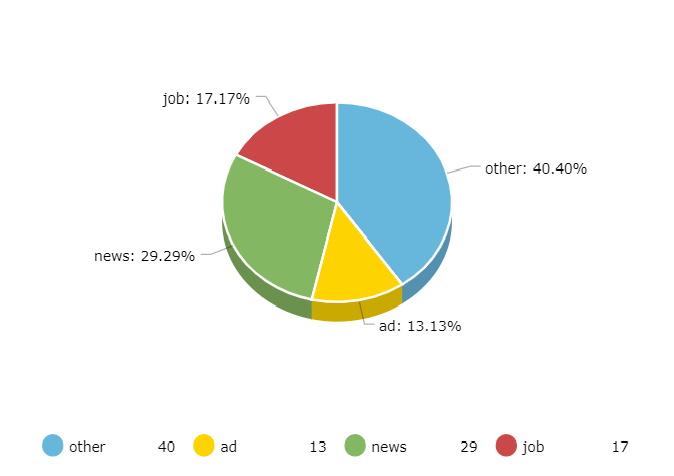
\includegraphics[width=\linewidth]{figures/Actual_Labeling}
    \caption{Actual Labeling}
\end{figure}
\vfill 
\clearpage

\newpage

\clearpage
\vspace*{\fill}

\subsection{Dictionary-Based Filtering Algorithm}
\large
{
\quad
Since the algorithm labels tweets based on several dictionaries of keywords, we can say that its manner of classification is a naïve one. \textbf{Moreover, the classification is strongly dependant on the order in which each dictionary is used.} For example, if a tweet contains keywords from 2 dictionaries, in our case \textbf{A} and \textbf{B}, depending on the order in which those dictionaries are verified, the tweet can be labeled as being from both \textbf{A} and \textbf{B}. 
}

\begin{figure}[H]
    \centering
    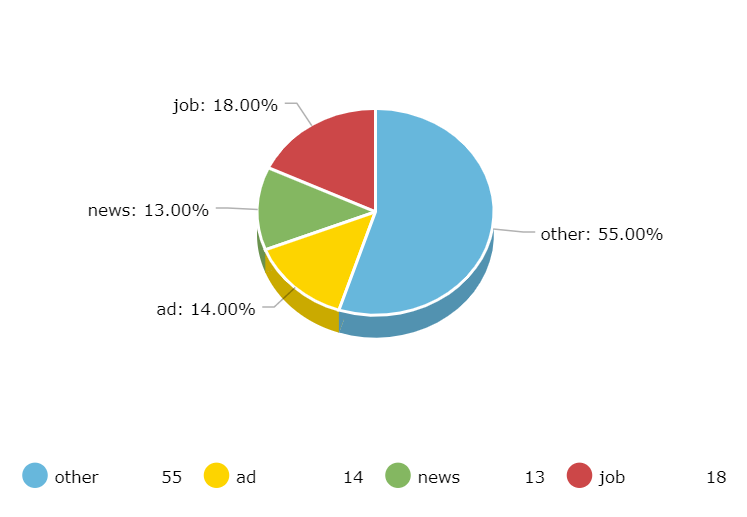
\includegraphics[width=\linewidth]{figures/DictionaryBasedAlg}
    \caption{Dictionary Based Algorithm}
\end{figure}

\vfill 
\clearpage
\newpage

\clearpage
\vspace*{\fill}

\subsection{Naive Bayes Algorithm}
\large
{
\quad
In order to work, the algorithm makes use of a sample training data pool. Because of that, \textbf{the precision of the classification is dependant on the size and variety of the sample pool.} The larger the sample pool, the better the results, but if the sample pool is lacking variety, then classification errors are still bound to occur. For example, the \textit{news} label can be assigned to tweets commenting or expressing opinions on different news.
}


\begin{figure}[H]
    \centering
    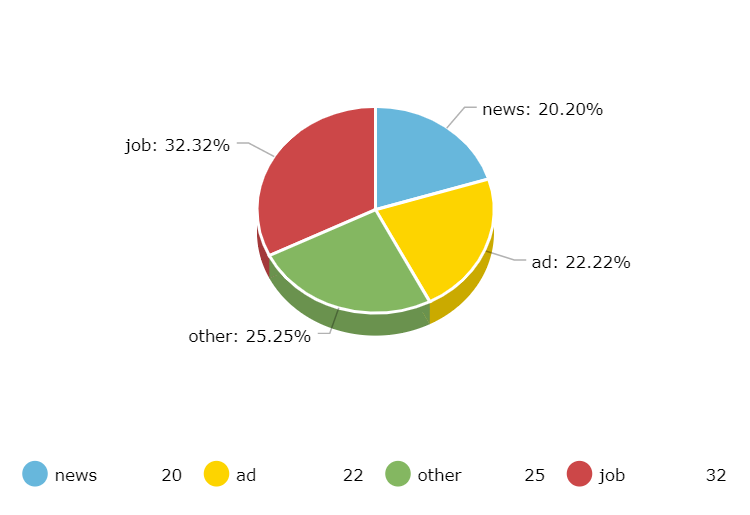
\includegraphics[width=\linewidth]{figures/NaiveBayes}
    \caption{Naive Bayes Algorithm}
\end{figure}

\vfill 
\clearpage
\newpage

\section{Conclusion}
\large
{
\quad
Taking all the above into account, we can say that a Naive Bayes approach for a classification algorithm is generally favorable. Unlike a keyword based filtration algorithm, which makes use of one or many dictionaries in order to classify the tweets into different categories (because of that, it can often fail), a Naive Bayes algorithm works with training data, meaning that it labels the received tweets with respect to a population of already labeled tweets. Therefore, even if a misleading tweet might have corresponding keywords or tags, it can be correctly classified based on the algorithm's training data. The downside to this is the required amount of training data. In order to reach satisfactory results, one should provide a large number of already correctly labeled tweets as data.
}

\begin{thebibliography}{1}

\bibitem{introduction}
    Classification of tweets into various categories using classification methods
    \url{https://www.ijariit.com/manuscripts/v4i3/V4I3-1505.pdf}
    
\bibitem{naive_property}
    Understanding Naive Bayes \& its applications in text classification
    \url{https://heartbe.fritz.ai}
\end{thebibliography}

\end{document}